\subsection{MetaPath}

In MetaDE package,
following the detection of biomarkers, pathway analysis (a.k.a. gene set enrichment analysis) is usually performed for functional annotation and biological interpretation. 
Beyond that, the MetaPath module provides two advanced meta-analytic pathway analysis tools: 
Comparative Pathway Integrator (CPI) and Meta-Analysis for Pathway Enrichment (MAPE) (Shen et al., 2010; Fang et al., 2017). 
Pathway clustering with statistically valid text mining is included in the package to reduce pathway redundancy to condense knowledge and increase interpretability of clustering results. 
The R package for MetaPath module can be found \url{https://github.com/metaOmics/MetaPath}.

\subsubsection{Procedure}
The MetaPath package requires the input of raw expression data as in MetaDE. 
There are three major steps to implement the package: pathway analysis, pathway clustering diagnostics and pathway clustering with text mining. 
As shown in Figure \ref{fig:MetaPathoption}, there are 9 major options that need to be specified to implement the package.
Detailed list of all options available for the package can be found at the end of this subsection. 


\begin{figure}[H]
\begin{center}
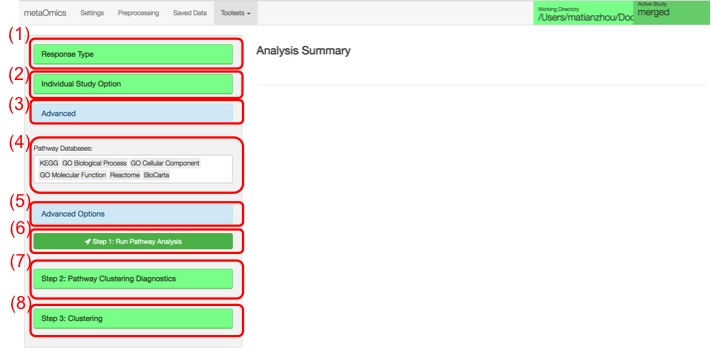
\includegraphics[scale=0.5]{./figure/metaPath/metaPathoption.pdf}
\caption{``MetaPath" options}
\label{fig:MetaPathoption}
\end{center}
\end{figure}

\begin{steps}
\item \textbf{Setup pathway analysis parameters:}
Users need to specify {\color{red}(1) } whether the input gene expression profile is mixed of continuous data and discrete data;
{\color{red}(2)} response type, case/control labels (similar to MetaDE);
{\color{red}(3)} individual study option (similar to MetaDE);
{\color{red}(4)} advanced options including whether to adjust for covariates or the direction of hypothesis testing;.
In {\color{red}(5)}, users can select from 25 available pathway databases for the enrichment analysis.
In {\color{red}(6)}, users can select MetaPath method (either CPI or MAPE).
By default, the ``CPI" approach is used, otherwise ``MAPE" approach can also be used. Other options include pathway enrichment method (the Fisher's exact test or KS test), the minimum and maximum pathway size. If ``Fisher's exact test" is chosen for the enrichment method, users need to further specify the criteria for selection of DE genes, e.g. the number of top ranked genes. On the other hand, if ``KS test" is chosen, one needs to further specify whether to use permutation to obtain enrichment p-value. 

\item \textbf{Run Pathway Analysis:}
\label{step:metaPath1}
Once the above options are specified, users can click on {\color{red}(7)}, ``Run Pathway Analysis".

\textbf{Pathway clustering diagnostics:} 
\label{step:metaPath2}
From the previous step (Step~\ref{step:metaPath2}), users can choose the top enriched pathways for further clustering. 
One can expand the drop-down menu and use FDR cutoff to choose top pathways and click on {\color{red}(8)}, ``Pathway clustering diagnostics" to implement the second step.

\textbf{Pathway clustering with text mining:} 
\label{step:metaPath3}
From the previous step (Step~\ref{step:metaPath3}), users can determine the optimal number of clusters in the pool of pathways selected. 
Now, one can specify the number of clusters and click on {\color{red}(9)} ``Get clustering result". 
Note that you may not want to select too large $K$ since you wish to have a certain amount of pathways in each cluster for the validity of text mining algorithm. 
We generally suggest users to specify $K$ no larger than 7 for fewer than 100 pathways. 
\end{steps}





\textbf{Complete List of Options:} 

\begin{enumerate}
  \item mixed data types: whether the input data is a mixture of count data and continuous data.
  \item Response Type:
   \begin{itemize}
     \item Two class comparison, Multi-class comparison, Continuous outcome, Survival outcome.
     \item Label Attribute: select the label name of the outcome.
     \item Control Label \& Experimental Label: specify the case/control label for two-class comparison.
    \end{itemize}
   \item Individual Study Option:
     \begin{itemize}
     \item Setting individual study method
     \item Setting individual study paired option
    \end{itemize} 
   \item Advanced Option (**Optional):
     \begin{itemize}
      \item Covariate
      \item Alternative hypothesis
    \end{itemize} 
    \item Pathway Databases
    \item Pathway Analysis Option:
         \begin{itemize}
       \item Software
      \item Pathway enrichment method
      \item Pathway min gene size
      \item Pathway max gene size
    \end{itemize} 
    \item Run Pathway Analysis
    \item Pathway Clustering Diagnostics
    \item Get Clustering Result
\end{enumerate}


\subsubsection{Results}

\begin{figure}[H]
\begin{center}
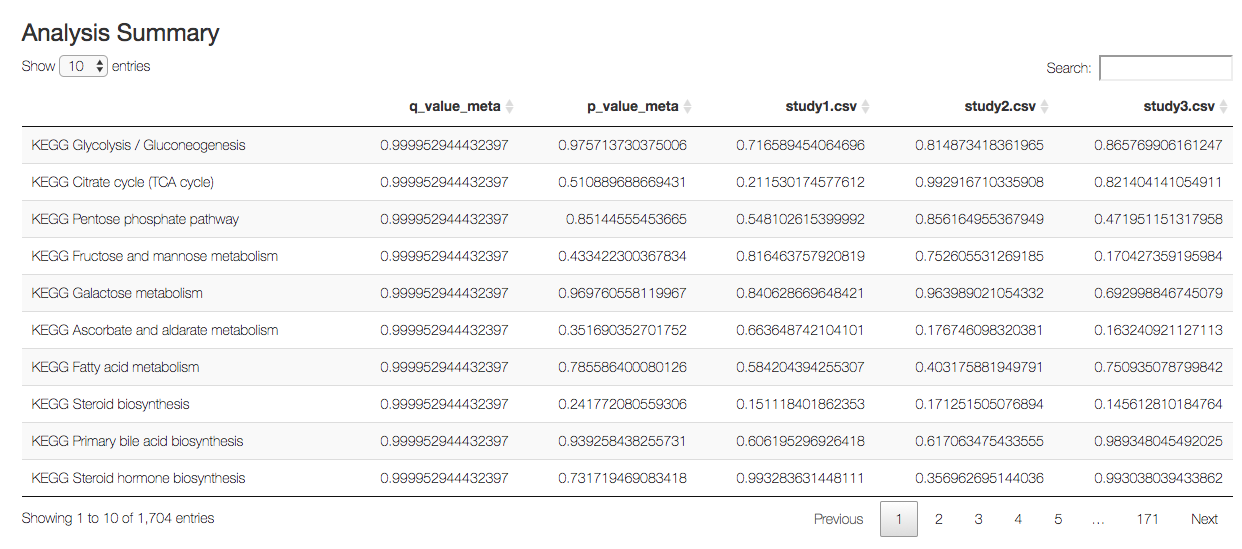
\includegraphics[scale=0.4]{./figure/metaPath/metaPathresult1.png}
\caption{``MetaPath" Results (1)}
\label{fig:MetaPathresult1}
\end{center}
\end{figure}

The input dataset is same as the input for MetaDE module.
We used multi-study leukemia gene expression data as example.
After performing merging of the three datasets and filter 50\% genes by mean and 50\% by variance, 1283 genes remained.
In this example we only compare two phenotypes: inv(16) and t(15;17).
Detailed descriptions of these studies can be found in Table~\ref{tab:realDataLeukemia}. 
After the Step~\ref{step:metaPath1} is finished, a summary table was generated as shown in Figure~\ref{fig:MetaPathresult1} (based on the default CPI method). The ``Analysis Summary" includes the analysis results of all pathways, including individual study association analysis p-value, meta pathway analysis p-value/FDR, etc. Users can search the gene name in the ``Search" bar, and the full table is automatically saved in the working directory specified before.  

\begin{figure}[H]
\begin{center}
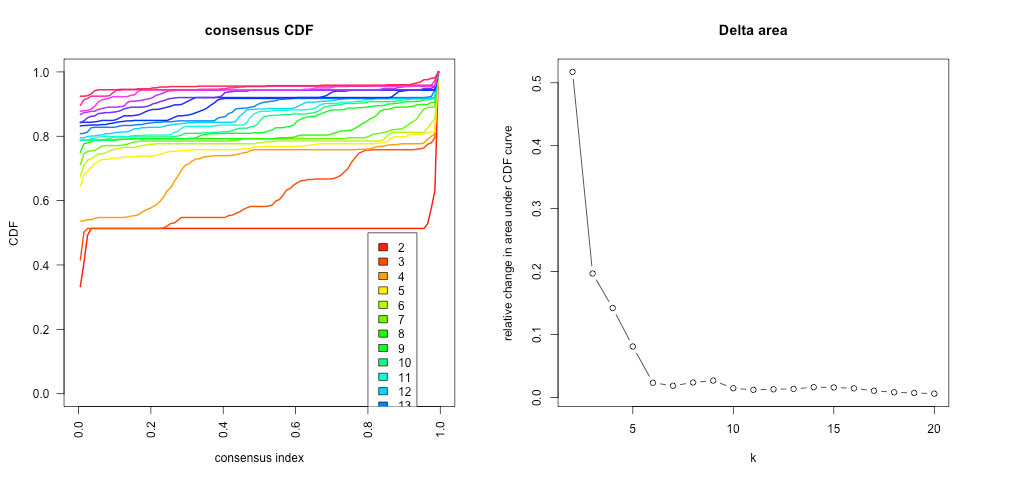
\includegraphics[scale=0.5]{./figure/metaPath/metaPathresult2.png}
\caption{``MetaPath" Results (2)}
\label{fig:MetaPathresult2}
\end{center}
\end{figure}

After the ``Pathway Cluster Diagnostics" step is finished, we will see two plots generated on the right panel (Figure \ref{fig:MetaPathresult2}): consensus CDF and Delta area plots, both from the ``ConsensusClusterPlus" package. The CDF of the consensus matrix for each $K$ (indicated by colors) is estimated by a histogram of 100 bins. The CDF
reaches an approximate maximum, thus consensus and cluster confidence is at a maximum at this $K$. The delta area shows the relative change in area under the CDF curve comparing $K$ and $K - 1$, thus allows users to determine the determine $K$ at which there is no appreciable increase in CDF. Both plots assist users in finding the optimal number of clusters $K$ and you may refer to (Monti et al., 2003) for more detailed interpretation of the two plots. In the demo example, $K=6$ has large enough CDF, is thus chosen (though $K=7$ captures more, we only have 38 pathways here). 

\begin{figure}[H]
\begin{center}
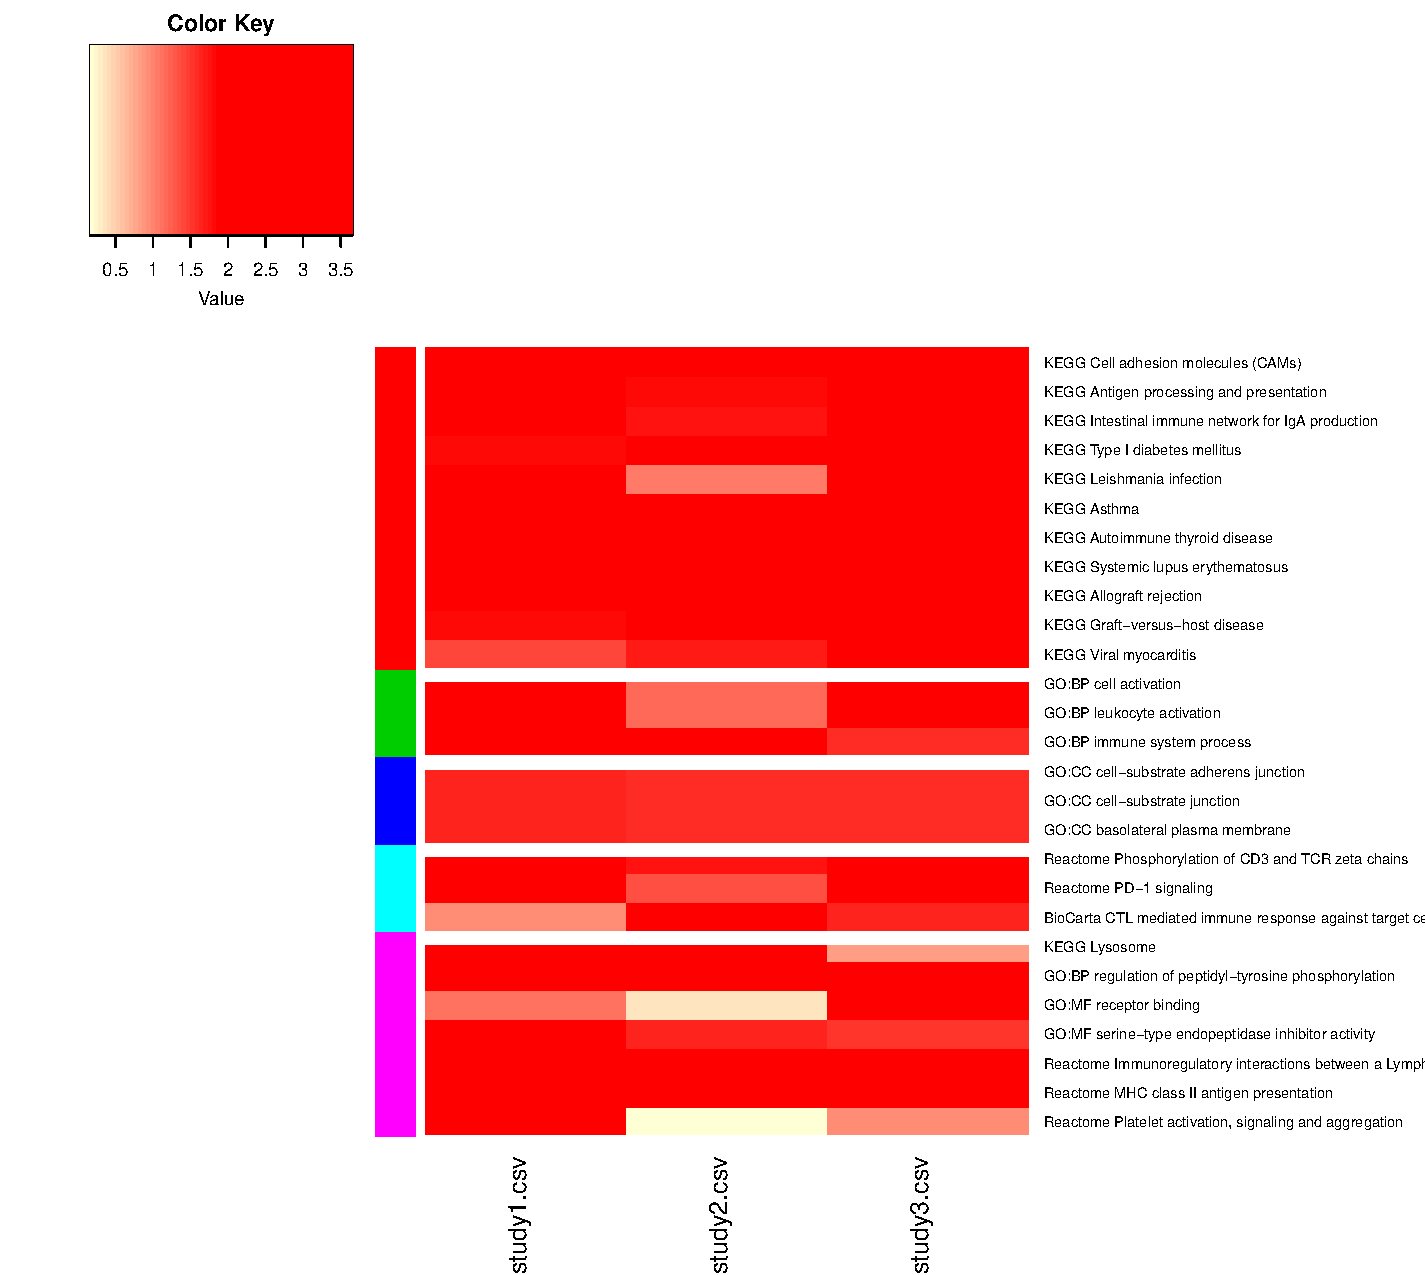
\includegraphics[scale=0.6]{./figure/metaPath/Heatmap_clusters_all.pdf}
\caption{``MetaPath" Results (3)}
\label{fig:MetaPathresult3}
\end{center}
\end{figure}


The heatmap in Figure~\ref{fig:MetaPathresult3} shows the -log10 transformed p-value of enrichment analysis in each study from \ref{step:metaPath1}. 
Studies are on columns and the selected pathways are on rows, red means more enriched. The pathways are sorted by the pathway cluster as indicated by the colors on the left side of the heatmap. 
In addition, 
the key words of each cluster of pathways are extracted and analyzed by a built-in text mining algorithm and one file named ``Clustering\textunderscore Summary.csv" is saved to the working directory which shows a summary of the text mining result. 



